\section{Semaine 4 - 26 fev}

\subsection{Lundi}

L'\textbf{objectif} d'aujourd'hui c'est de
\begin{itemize}
    \item Optimiser la bowtie simple
    \item Optimiser la bowtie vraie
    \item Optimiser la dipole
\end{itemize}

Pour les simulations, on a maintenant ajouté une couche d'oxide SiO$_{2}$. C'est cela qu'on voit dans la figure \ref{fig:oxide_film}.

\begin{figure}[h!]
    \centering
    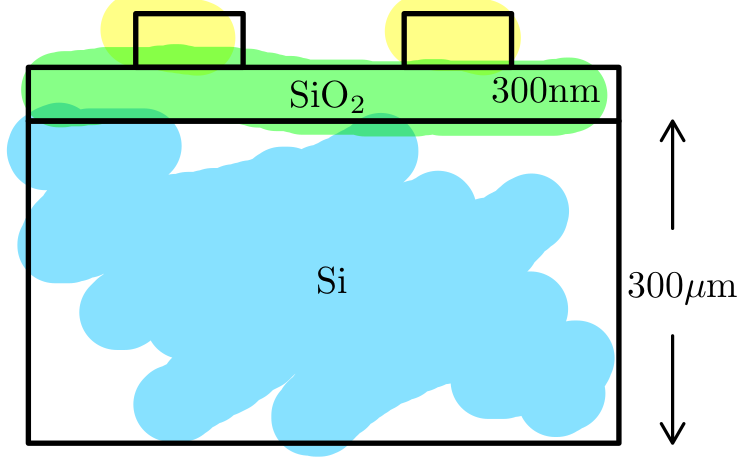
\includegraphics[width=0.35\textwidth]{texfigures/ocide_film.png}
    \caption{\label{fig:oxide_film} On ajoute une couche d'oxide au-dessus du substrat.}
\end{figure}

Les valeurs obtenus à travers CST son visibles dans la Table \ref{tab:parameters}



\begin{table}[h!]
    \centering
    \begin{tabular}{|c|c|}
        \hline
        Parameter & Value ($\mu$m) \\
        \hline
        Ec & 45 \\
        La & 246 \\
        Ea & 123 \\
        Le & 10 \\
        \hline
    \end{tabular}
    \caption{Parameters and their values in micrometers.}
    \label{tab:parameters}
\end{table}

\subsection{Mardi}

Mardi à été le jour de la session de nanofabrication. 